\documentclass[12 pt , twoside, letterpaper] {article}
\usepackage{geometry}
\newgeometry{margin=1.5cm}
\usepackage{amsmath}
\usepackage{amsfonts}
\usepackage{amssymb}
\usepackage{graphicx}
\usepackage[normalem]{ulem}
\renewcommand{\vec}[1]{\mathbf{#1}}
\let\oldhat\hat
\renewcommand{\hat}[1]{\oldhat{\mathbf{#1}}}
\usepackage{wasysym}     

\begin{document}
\title{Giancoli Ch19: Heat and the First Law of Thermodynamics}
\date{}
\maketitle
\vspace{-78pt}
\section{Heat as Energy Transfer}
	\begin{itemize}
		\item Heat is not a substance (the failed caloric theory)
		\item 1 calorie(cal)\footnote{1kcal= Calorie}= amount of energy required to raise the 				temperature of 1 kg of water by 1 degree celsius\footnote{Also British Thermal Unit 				(BTU)= The amount of energy required to raise the temperature of 1lb of water by 1 				degree F}
		\item Heat: energy transferred $\because \Delta$ temperature
		\item SI unit of heat: Joules  
		\item Mechanical equivalence of heat: work done$\rightarrow$ increase in temperature (1 cal = 4.186 Joules)
	\end{itemize}

\section{Internal Energy}
	\begin{itemize}
		\item Internal (Thermal)  Energy: total energy of all molecules
		\item Temperature: measure of average thermal $E_k$ of individual molecules
			\footnote{Remember that heat is ONLY dependent on temperature}
		\item Internal Energy of an Ideal Monoatomic Gas
			Assumptions:
			\begin{enumerate}
			\item If more than one atom in a molecule than need to consider rotational$E_k$ ,vibrational $E_k, E_p$. But still only $\alpha$ on T		
			\item Real Gas: largely dependent on T but also has a bit of dependence on P,V
			\item Liquid, Solids: Complicated Internal energy$\because$ take into consideration 					electrical bond energy
			\end{enumerate}
			\begin{align}
				E_{int}=\Sigma E_{k\quad translational}&=N(\frac{1}{2}m\overline{v}^2)
																			\\&=N(\frac{3}{2}kT)		
																			\\&=\frac{3}{2}nRT
			\end{align}
	\end{itemize}
\section{Specific Heat}
	$$Q= mc\Delta T$$	
	\begin{itemize}
		\item for solids and liquids, the value of c somewhat dependent on T and a bit on P
		\begin{align*}
		\because \text{c is a function of T}\rightarrow c(T)\text{we write heat as:}&
		&\\dQ=mc(T)dT \quad\quad \rightarrow\quad
		Q=\int^{T_2}_{T_1}mc(T)dT
		\end{align*}
		\item but for $\Delta T \rightarrow 0$ we treat c as constant
		\item Gas more complicated
	\end{itemize}
	
\section{Calorimetry}
	\begin{itemize}
		\item Closed system: no mass in or out (but can energy exchange)
		\item \textbf{Isolated} system if no energy in or out of its boundaries
		\item Isotropic tendency within system
		\item Conservation of energy valid for  isolated closed sys (often if not $\rightarrow$ approx )
		\item heat gained = heat lost
		\item Consider all sources of energy transfer
		\item Calorimetry : quantitative measurement of heat exchange
		\item ``method of mixtures" : calculate specific heat by mixing 
	\end{itemize}
	
\section{Latent Heat}
	\begin{itemize}
		\item is the energy released or absorbed by a system during a constant temperature process. 
		\item Typical ex. is energy involved in change of phase 
		\item Heat of fusion ($L_f$): heat required to change 1 kg of substance (s) $\rightarrow$ (l)
			\footnote{$L_f, {water} = 3.33 \times 10 ^5 J/kg$}
		\item Heat of vaporization ($L_v$) : heat required to change 1 kg of substance (l) $\rightarrow$ (g)
			\footnote{for water, 2260 kJ/kg}
		\item heat involved in phase change= Q =mL where L: latent heat of the particular process and substance
		\item The value of $L_v$ increases slightly with a decrease in temperature.(?)
	When water evaporates, since the energy required comes from the water itself ($L_v$) so its internal energy $\therefore$ T $\downarrow$. (ex. sweating)
		\item Energy is used for bond breakage/ formation in molecules instead of used to increase average kinetic energy. And $\because$  (l) $\rightarrow$ (g) is a more violent reorganization than (s) $\rightarrow$ (l) $\therefore$usually $L_v >L_f$
	\end{itemize}		

\section{The First Law of Thermodynamics}
	\begin{itemize}
		\item heat : transfer of energy due to a difference in temperature
 		\item work : transfer of energy tat is not due to a temperature difference
 		\item First law of thermodynamics 
 				\begin{equation}
					\Delta E_{int} = Q - W		
				\end{equation}				 		
 		\\where Q: net heat \textbf{added} to the system
 		\\ W: net work done \textbf{by} the system
 		\item restatement of conservation of energy $\rightarrow$ applies only to closed system
 		\item if open system, must taken into account the internal energy due to increae of decrease in the amount of matter.
 		\item Isolated system : W=Q=0 (no heat or work on sys) $\therefore E_{int}=0$
 		\item State variable: describe the state of a system 
 			\footnote{Q , W are NOT state variables}
 		\item Also useful to write as $dE_{int} $= dQ - dW
 			\footnote{dQ and dW are not exact differential}
 		\item For a \textbf{moving} system with potential energy,
 		\begin{equation}
 		\Delta K + \Delta U +\Delta E_{int}=Q - W
 		\end{equation}
	\end{itemize}
	\section{Work Calculation}
	Area under PV graph:
	\begin{figure}
				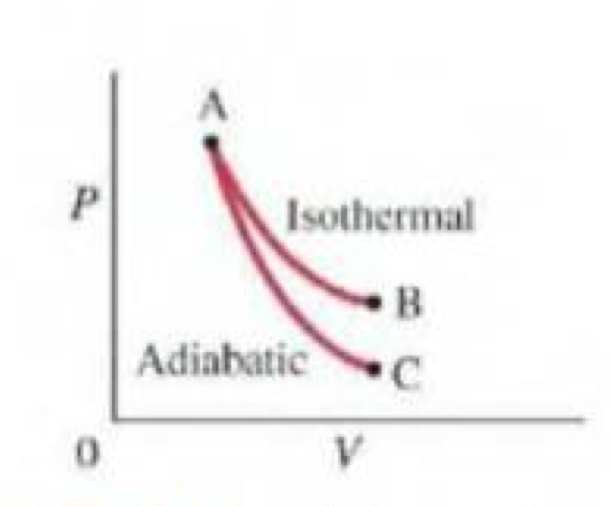
\includegraphics[scale=0.5]{AdIso}
				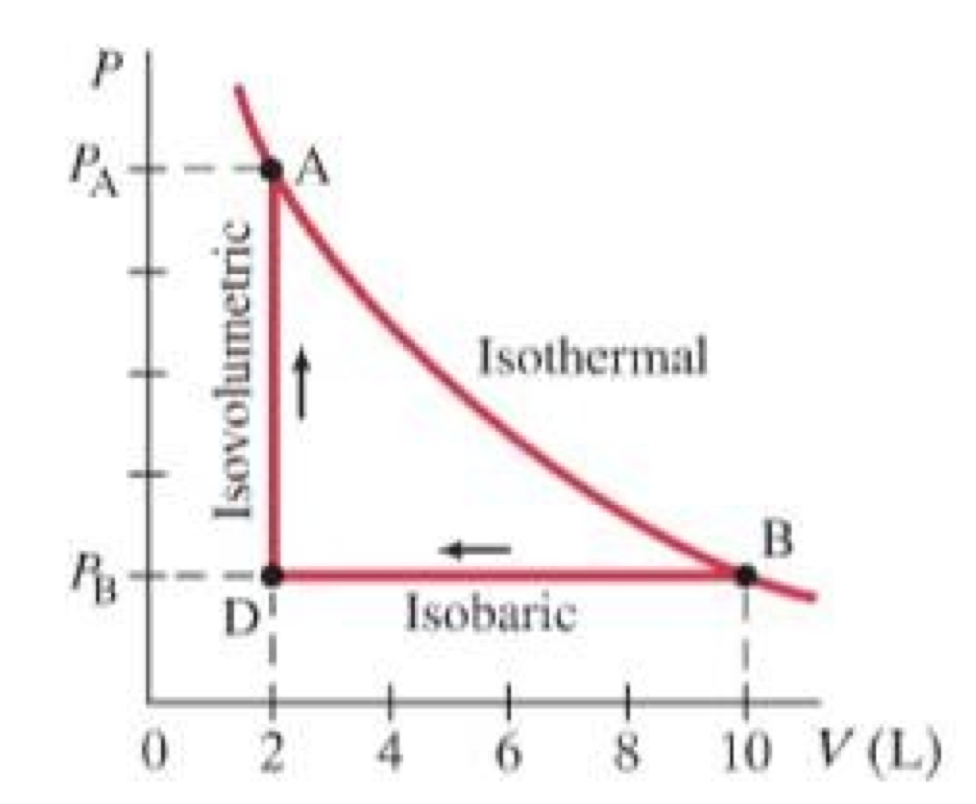
\includegraphics[scale=0.3]{PVdiag}	
	\end{figure}
		\subsection{Isothermal processes $\Delta $T=0}
		\begin{itemize}
		\item Isotherm : curves on isothermal PV graph
		\item Ideal gas $\therefore$ PV= constant at every point on graph 
		\item Heat reservoir: a body whose mass is so large that T $\approx$ constant when heat is exchanged
		\item quasistatically : moving so slow (i.e. static) that T doesn't signficifantly change 
		\item $E_{int}=\frac{3}{2}nRT \because$ mass, T unchanged $\therefore E_{int}$ unchanged
		\\ $E=Q - W=0 \quad \rightarrow \quad Q=W$
		\\ work done by gas in an isothermal process = heat added to gas
		\end{itemize}
		\subsection{Adiabatic Processes (Q=0)}
			\begin{itemize}
				\item situation: short $\Delta t$ or well insulated 
				\item $\because$ 1st law of thermo : $\Delta E_{int} = - W$ 
				\item ex) Adiabatic compression $\rightarrow$ T $\uparrow \rightarrow$ Diesel fuel mixture ignite spontaneously \footnote{1st law of thermo also holds for Isobaric and Isovolumetric (Isochoric) Processes }
			\end{itemize}
			
		\subsection{Work Done in Volume Changes}
		Work and heat are not property of a system, they are not only dependent on final and initial but also depend on type of process (``path independent")
		$dW=\vec{F} d\vec{l}= PA d\vec{l}= PdV$ where $d\vec{l}$ point into the gas
\\		Isobaric
			\begin{itemize}
				\item Area under PV graph is rectangle $W=P(V_f-V_i)$
				\item as volume change in gas, P=$P_b$ throughout $\rightarrow P=\frac{nRT_b}{V_b}$
				\item divide both side by $V_b \rightarrow \therefore W= nRT_b(1-\frac{V_a}{V_b}$
				\footnote{Remeber to always define what exactly is our system}
			\end{itemize}
		Isothermal
			\begin{align}
				W= \int dW=\int PdV= nRT ln \frac{V_b}{V_a}
			\end{align}
			Free Expansion
			\\ 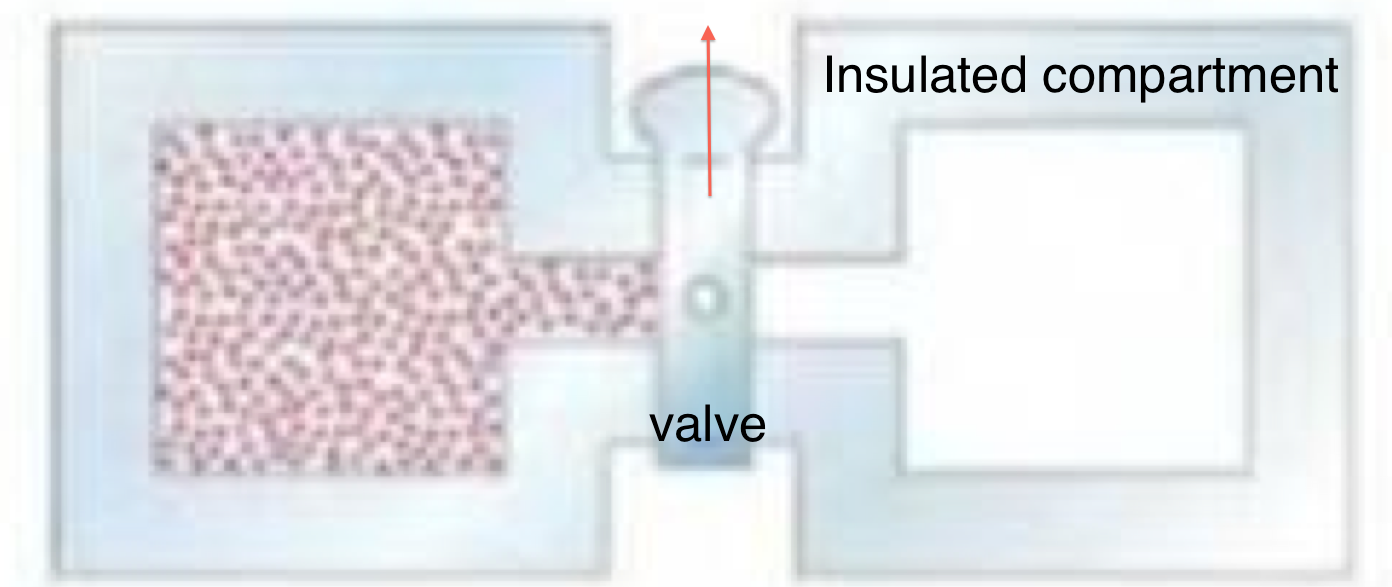
\includegraphics[scale=0.2]{FreeExpansion}
			\begin{itemize}
				\item a method of adiabatic expansion with W=0
				\item release valve: gas move from one compartment to another 
							$\because$ gas does not move any obj $\therefore$ W=0
				\item $\therefore$ by 1st law $\rightarrow \Delta E_{int} =0 \rightarrow \Delta T=0$
				\item Using this method, we experimentally show that $\Delta T \rightarrow 0 \text{ but} \neq 0 \therefore \Delta E_{int}$ does not depend solely on T but also a bit on P and V
				\item Rapid process \footnote{instead of being quasistatic} $\therefore$ state variables in intermediate stages are not well define $\rightarrow$ can not be plotted on PV diagrams 
			\end{itemize}
	\section{Molar specific heat for gas Equipartiton of E}
		\begin{itemize}
			\item molar specific heat (C): heat required to raise 1 mol of gas by 1 deg Celsius @ constant V \& P
			\item depend on process : isobaric ($C_p$) ,isochoric ($C_v$)
				$Q=nC_v\Delta T$ \footnote{ditto for $C_p$ for these equ in this section}
			\item$ M= molar mass= \frac{m}{n}=[\frac{g}{mol}]$			
			\item $C_v= Mc_v$
			\item value of C are $\approx$ same for different gas wih same \# of atoms per mcl
		\end{itemize}
		\subsection{$C_p -C_v=R$}
			\vspace{15cm}
		\subsection{Equipartition of Energy}
		\begin{itemize}
			\item more \# of atoms in mcl $\rightarrow$ more Degrees of freedom $\rightarrow$  molar specific heat $\uparrow$
			\item \textbf{Principle of equipartiton of Energy}: 
					energy is shared equally among the active Dof and each active Dof of a mcl has $E_{avrg}= \frac{1}{2}kT$
			\item Diatomic: 3 Dof translational +2 Dof rotational
			\item @ high T: diatomic gas has 2 new Dof from electrical,spring-like,vibrational $E_k \rightarrow C_{\text{v,diatomic}}=\frac{7}{2}$
			\item @ low T : almost no $E_k$ rotational $\rightarrow$ 3 Dof
			\item this phenomenom is explained by Brownian motion , which gives molecules its discrete nature. Discrete Dof at discrete T $\rightarrow$ quantized minimum energy
			\item Can apply princple of equipartition to solids too!
			\item $C_{\text{any solid @ high T }}\approx $Dulong and Petit value= 3R
			\\ $\because 3 E_k + 3E_p$ spring-like in crystalline structure
		\end{itemize}
	\section{Adiabatic Expansion of gas}
Deriving relation between P and V of quasi-static adiabatic expansion of an ideal  gas
	\vspace{15cm}
	
	\section{Heat Transfer}
		\subsection{Conduction}
			\begin{itemize}
			 \item transfer of $E_k$ through molecular collisions
			 \item \begin{equation}
			 \frac{dQ}{dt}= - kA\frac{dT}{dx}
			 \end{equation}
			 \item negative sign $\because$ Q flow is opposite to direction of temperature gradient
			 \item conductor: large k ; insulator : small k
			 \item Thermal resistance (R-value): measure of thermal property in building material:
			 $R=\frac{thickness}{k}$
			\end{itemize}

		\subsection{Convection}
			\begin{itemize}
				\item heat flow by mass movement of large number of molecules over large distances
				\item forced convection (ex: forced-air furnace)
				\item Natural convection $\because$ density difference
			\end{itemize}
		\subsection{Radiation}
			\begin{itemize}
				\item doesn't require matter as medium
				\item rate at which an object radiates energy $\alpha \quad \quad T^4$
				\item Stefan-Boltzmann equation :  $\sigma$=Stefan-Boltzmann constant=$5.67 \times 10^{-8} W/m^2 \cdot K^4$
					\begin{equation}
						\frac{\Delta Q}{\Delta t}=\epsilon\sigma A T^4					
					\end{equation}
				\item $\epsilon$= emissivity (0$\leq  \epsilon \leq1$)
						\begin{itemize}
							\item somewhat $\alpha$ on T
							\item good emmiter (dark)L absorb almost all radiation ($\epsilon\approx1$)
							\item obj not only emit but also absorb radiated energy $\therefore$good emmitter is also a good absorber
							\item Opposite: shiny surfaces
						\end{itemize}
						\item obj emmit $\rightarrow$ surrounding absorb $\rightarrow$ surrounding emmit\\
							$\therefore $Net rate radiant heat flow from obj= $\frac{\Delta Q}{ \Delta t}=\epsilon\sigma A (T_1^4- T_2^4) $where $T_2$ temp of surroundings
							\item we can't use this to calculate Sun's radiant heat , $\because$ Sun is point source not a ``surrounding"
							\item Solar constant= amount of energy from Sun striking Earth's atmosphere =1350 W$/ m^2$
							\begin{equation}
							\frac{\Delta Q}{\Delta t}=(1350 W/ m^2) \epsilon A cos\theta
							\end{equation}
							where $\theta$ =angle between Sun's rays and the area's normal
							\item ex) seasons, thermography
			\end{itemize}
	\section{Question}
		\begin{enumerate}
			\item  pg 526 	The value of $L_v$ increases slightly with a decrease in temperature.(?) What is the prupose of this anyways? if water only evaporate at 100 degree, why should we care about $L_v$ at other temperature?
		\end{enumerate}
\end{document}